\documentclass[a4paper,11pt]{article}

\usepackage{fullpage}%
\usepackage[T1]{fontenc}%
\usepackage[utf8]{inputenc}%
\usepackage[main=francais,english]{babel}%
\usepackage{amsmath}
\usepackage{algorithmique}

\usepackage{graphicx}%
\usepackage{url}%
\usepackage{abstract}%

\usepackage{mathpazo}%

\usepackage[backend=biber]{biblatex}%
\bibliography{papers}% The name of your .bib file

\parskip=0.5\baselineskip

\sloppy


\begin{document}

\title{Identification de problèmes SAT caractéristiques}%
%\thanks{Le fichier source est disponible à la référence~\cite{canevas}.}%

\author{Antonin Garret}

\date{12 juillet 2016}

\maketitle

\begin{center}
Merci à Laurent Simon
\end{center}

\begin{abstract}
La résolution de problèmes SAT trouvent une utilité croissante dans de nombreux domaines industriels, où de nombreux problèmes peuvent être réduits à une instance de SAT.
De nombreux programmes, les SAT-Solvers, sont développés et améliorés en continu pour résoudre toujours plus d'instances du problèmes avec les meilleurs performances possibles. Cependant ces amélioration passent par un processus expérimentale qui consiste à tester les SAT-Solvers sur une grand ensemble de problèmes, demandand un temps de calcul très élevé.
L'objectif de ce travail est de déterminer une classification des différentes instances du problème, pour rechercher des groupes de problèmes plus réduits sur lesquels une amélioration des performances d'un solveur se traduirait avec une forte probabilité par une amélioration des performances sur une catégorie dans sa globalité
   
  \begin{description}
  \item[Mots-clés:] 
  Problèmes SAT
  SAT-Solvers
  Machine-learning
%\item[Classification ACM:] Voir les codes à l'adresse
%  \begin{center}
%    \url{http://www.acm.org/about/class/class/2012}.
%  \end{center}

  \end{description}
\end{abstract}

\section*{Introduction}
Le problème de satisfiabilité des formules logiques, ou problème de décision SAT, fut l'un des premiers problème à être prouvé NP-complet. En conséquence, il fut longtemps considéré qu'une fois un problème réduit à SAT,
il était inutile de le chercher à le résoudre en raison de la NP-complétude ainsi démontrée. Cependant, l'abandon de la recherche d'une résolution complète et le choix d'une approche plus expérimentale du
problème ont conduit à la création dans les dernières décennies de nombreux programmes, appelés SAT-solvers, qui permettent de résoudre une portion toujours grandissante des instance du problème en un temps 
raisonnable. Ainsi, de nos jours, réduire un problème à SAT signifie que l'on a de grande chances de l'avoir déjà résolu.

Hors de nombreux problèmes industriels sont réductibles à SAT. ce qui motive la recherche constante d'une amélioration des performances des SAT-solvers qui trouvent ici une application directe. 
Cette recherche d'amélioration vise avant tout ces problèmes industriels, amis aussi des instances générées aléatoirement ainsi que d'autres crées à partir de problèmes logiques classiques. Les performances 
des solveurs sont donc régulièrement testées sur de grands ensembles de problèmes, des benchmarks, qui sont témoins de l'évolution de l'état de l'art des solveurs. Ces tests permettent un vérification par 
l'expérience de l'efficacité des méthodes utilisées pour résoudre les différents problèmes, mais elle présente l'inconvénient majeure de demander un temps de calculs très élevé, car il faut effectuer des tests
sur un grand nombre de données. L'objectif de ce travail est donc de chercher des moyens de minimiser cet inconvénient, en établissant dans un premier temps des classes de problèmes sur lesquels le comportement 
des différents solveurs est similaire, ce qui pourrait permettre de trouver des informations supplémentaire sur l’évolution d'un solveur, 
puis en recherchant des problèmes "caractéristiques" des ces classes, sur lesquels une amélioration des performances d'un solveur se traduirait avec une forte probabilité par 
une amélioration des performances sur l'ensemble de la classe, ce qui économiserait un temps de calcul non négligeable lors des phases de test.


\begin{itemize}
\item Les SAT-solver
\item Problème induit par l'amélioration par itération des programmes
\item Identification de problèmes caractéristiques
\item Plan du rapport, avec des renvois symboliques comme ceci: voir la
  section~\ref{sec:description}.
\end{itemize}

\section{Description du domaine}
\label{sec:description}

\subsection{SAT-Solver}

\subsubsection{Présentation du problème SAT}
Une formule logique est une formule composée de variables booléennes liées par l'algèbre booléenne. Un littéral est variable aléatoire ou sa négation. Une valuation est l'assignation d'une valeur à chacune de ces variables. Le problème SAT consiste à déterminer 
s'il existe pour une formule logique donnée une valuation qui la satisfait, c'est à dire pour laquelle cette formule devient vraie. Ce problème fut prouvé NP-complet par Stephen Cook et Leonid Levin au début 
des années 1970. 

La majorité des SAT-solvers prennent en entrée des problèmes sous forme normale conjonctive, ou CNF, c'est-à-dire sous la forme d'une conjonction de clauses composées d'une disjonction de littéraux. 
Il est possible de faire passer n’importe quelle formule en forme normale conjonctive, et ceci en un temps linéaire si l'on consent à ajouter des variables, cette contrainte n'a donc que peu d'importance lors 
de la résolution de problèmes réels.

La plupart des solveurs modernes se basent sur l'algorithme DPLL (pour Davis–Putnam–Logemann–Loveland). L'idée générale de cet algorithme est de choisir assigner une à une des valeurs à chaque variable, en 
effectuant un backtracking lorsque l'on abouti à une évaluation qui rend la formule fausse. Il utilise les deux principes suivants pour améliorer cette recherche d'une valuation correcte :

\begin{itemize}
	\item Propagation des clauses unitaires : si une clause est unitaire, c'est-à-dire qu'elle ne contient qu'un seul littéral, alors la valeur vrai doit être assignée à ce littéral, car sinon la clause en 
	elle-même ne pourrait pas être vraie.
	\item Élimination des littéraux pures : une variable qui apparaît dans la formule sous forme positive uniquement, ou négative uniquement, est appelé un littéral pure. Le littéral peut donc être retiré sans incidence 
	car on peut le désigner comme vrai sans risquer de conflit.
\end{itemize}

On peut se rendre compte qu'une valuation, même partielle, ne satisfait pas la formule si après l'application de ces règles, on constate la présence d'une clause vide, qui ne contient plus aucun littéral. C'est 
à ce moment là qu'on effectuera le backtracking. En réalité, comme on peut le voir dans cette description de l'algorithme, il n'est pas nécessaire de garder en mémoire les assignations de chaque variable. 
L'assignation, grâce à la propagation des clauses unitaires, se fait directement en modifiant la formule. De même, le backtracking se produit automatiquement : en assignant les différentes variables, on crée un 
arbre de décision, et arriver à une clause vide renverra Faux et causera un retour à une branche plus haute de l'arbre.

\begin{pseudocode}[ovalbox]{DPLL}{\Phi}
\SI \Phi \text{ est composée uniquement de clauses unitaires } \RETOURNE {Vrai}\\
\SI \Phi \text{ contient une clause vide } \RETOURNE {Faux} \\
\POUR \text{chaque clause unitaire } c \in \Phi
\FAIRE \Phi \PREND \textit{propagation-unitaire}(c, \Phi)\\
\POUR \text{chaque littéral pur } l \in \Phi
\FAIRE \Phi \PREND \textit{assigne-litteral-pur}(l, \Phi)\\
l \PREND \textit{choisir-litteral}(\Phi)\\
\RETOURNE DPLL(\Phi \wedge l) \text{ ou } DPLL(\Phi \wedge \neg l)\\
\end{pseudocode}

Bien que la manière de choisir un littéral à assigner n'ait pas été précisée, on peut considérer dans un premier temps que ce choix se fait aléatoirement. Cependant cette première approche ne cherche pas à 
optimiser le traitement des variables, afin de diminuer le temps de calcul. Les solveurs à apprentissage de clauses basé sur le conflit, ou Conflict-Driven Clause Learning (CDCL), qui constitue la plus grande 
partie des SAT-Solvers Modernes, utilisent l'algorithme DPLL en utilisant des heuristiques qui leurs sont propres pour choisir quelles variables assigner, ainsi que pour opérer un backtracking non linéaire, c'est 
à dire que rencontrer un conflit n’entraînera pas un retour à la dernière assignation avant le conflit, mais à une étape choisie par l'heuristique. De plus certains solveurs ajoutent lors des retours en arrière 
des clauses "apprises" lors de ces conflits, qui doivent permettre d’accélérer la résolution ultérieur du problème. De manière générale, les solveur CDCL ne sont pas adaptés à prouver l'insatisfiabilité d'une 
formule, car leur méthode de résolution consiste à parcourir les différentes valuations pour chercher celle qui satisfait le problème étudié. Prouver l'insatisfiabilité d'une formule demanderait donc de vérifier 
qu'aucune valuation ne convient. Compte tenu du temps de calcul que cela représente, on préférera presque toujours arrêter les calculs au bout d'un certains laps de temps, et en conclure que le problème est insatisfiable. 
Cependant il existe alors une probabilité non nulle que la formule soit en réalité satisfiable.


\subsection{Glucose}

Le solveur Glucose, développe par Laurent Simon et Gilles Audemard, est un exemple de Solveur CDCL avancé qui a fait ses preuves en matière de performances ces dernières années.
Glucose est basé sur MiniSAT, un solveur créé en 2003 par Niklas Eén et Niklas Sörensson avec un code se voulant simple et minimaliste, le but déclaré étant de le rendre facile à reprendre et à améliorer, 
afin de facilité dans le futur la création de nouveaux solveurs sur une base commune. Plusieurs aspects de MiniSAT sont eux-même basés sur l'algorithme Chaff. Pour propager les informations relatives aux assignations, 
MiniSAT, plutôt que d'effectuer la propagation sur l'ensemble de la formule, ce qui peut se réveler assez lourd, utilisent des ensembles de contraintes (qui sont des ensembles de clauses) relatives à chaque variable. 
Ce sont donc ces contraintes qui généreront des conflits. Lorsqu'un conflit est détecté le programme utilise la contrainte qui est à son origine pour établir l'ensemble d'assignations de variables qui a conduit 
à ce conflit. A partir de cet ensemble est crée une clause qui est vraie uniquement cet assignation particulier n'est pas opéré, et on conserve cette clause en tant que clause apprise. Les clauses apprises 
permettent de détecter certains conflits beaucoup plus rapidement, ce qui accélère la recherche d'une valuation correcte. Cependant conserver un trop grand nombre de clauses apprises peut à terme ralentir la recherche 
c'est pourquoi le nombre de clauses apprises reste limité. De plus MiniSat utilise une heuristique basée sur un système d'activité afin de gérer les assignation : à chaque variable est liée un nombre qui représente son activité, et 
ce nombre est augmenté lorsque la variable est impliquée dans un conflit. L'activité de toute les variables décroît naturellement au fil du temps ce qui conduit au fait attendu que seule les variables étant régulièrement 
impliqués dans des conflits conservent une activité élevée. Il existe un système similaire relatif aux clauses apprises, qui permet de choisir quelles clauses garder lorsque la limite évoquée plus haut est atteinte. 


Glucose quant à lui est un des successeurs de MiniSAT. Parmi ceux-ci il existe un problème lié aux nombres de clauses apprises qui sont conservées. Pour résoudre certains problèmes difficiles, il est nécessaire garder un 
grand nombre de clauses, car on ne sait pas a priori quelle clauses se révéleront utiles. Cela présente une difficulté pour de nombreux solveurs, certains devant même capituler à cause de problèmes de mémoire. La 
démarche derrière Glucose était donc justement de trouver un moyen de détecter à l'avance les clauses qui seront les plus utiles. La méthode utilisée a été d'étudier les niveaux de décision des différents littéraux 
d'une clause, c'est à dire l'ordre dans lequel ils sont choisis par rapport au moments "d'activité" de la clause (quand elle entraîne une propagation ou un conflit). Il semble y avoir une relation entre la manière 
dont s'étend une clause sur ces niveaux de décision et son activité, donc son utilité. En particulier certaines clauses, appelées "glue clauses" repérées grâces à cette méthode semblent avoir une importance particulière. 
Ce sont elles qui donnent son nom au solveur. Glucose se sert de ces informations supplémentaires pour régulièrement réduire de manière drastique le nombre de clauses apprises. 
Afin d'éviter de se perdre dans une branche de l'arbre de décision qui peut se revéler infructueuse, Glucose effectue aussi des redémarrages, des "restarts" complets après un certain temps, c'est-à-dire un 
"backtracking" jusqu'à la racine de l'arbre.

Glucose a été publié en 2009, mais il a depuis continué à être amélioré à travers de nouvelles versions, ce qui lui a permis de rester parmi les solveurs les plus performants. Depuis 2014, il existe une version 
de Glucose, Glucose-Syrup, qui fonctionne sur des architectures parallèles.

\subsection{Benchmarks et competition SAT}

De part la NP-complétude du problème SAT, les SAT-Solvers ne peuvent pas résoudre toutes les instances de SAT en un temps raisonnable. Leur but est donc de résoudre un maximum de problèmes en en le moins de 
temps possibles. C'est pourquoi l'objectif de la recherche SAT est l'amélioration constante de ces solveurs et une grande quantité de temps est consacré à tester ces performances, seulement il est impossible 
de faire cela sur des problèmes créés à la volée. En effet, les SAT-solvers sont destinés à être utilisés sur des problèmes comptant plusieurs millions de littéraux et cela prendrait un temps énorme de créer 
des centaines de problèmes de cette taille pour tester un seul programme. De plus, la difficulté des problèmes varie grandement, et on ne peut pas prévoir quels problèmes seront utiles pour tester les performances 
d'un solveur. Enfin, les problèmes sur lesquelles il est le plus intéressant d'améliorer les performances sont les problèmes venant de l'industrie, il ne fait aucun doute, même si celles-ci ne sont pas identifiés,
qu'ils obéissent à certaines structures propres au milieu dont ils sont issus. 

Pour répondre à ce problème, des instances de grandes tailles, appelées benchmark. ont été mis à la disposition de tous. Ils en existe trois grandes catégories : les problèmes industriels, les problèmes aléatoires 
qui sont comme leur nom l'indique générés aléatoirement en influent sur différents paramètres, comme le rapport entre la taille des clauses et le nombres de variables, et les problèmes créés à partir de problèmes 
logiques classiques comme celui du cavalier. Les solveurs sont testés et re-testés sur ces benchmarks afin de mesurer les possibles améliorations introduites par les changements effectués. Cette méthode se rapproche 
beaucoup d'une approche expérimentale car de nombreux changements, parfois importants portant sur l'algorithme du solveur en lui-même ou parfois de simples test de nouvelles valeurs pour certains paramètres, sont 
introduits sans certitudes qu'ils provoqueront une amélioration des performances. Ils peuvent aussi n'avoir qu'une incidence sur une certaine catégorie de problèmes.

Les solveurs sont testés en grande partie sur les mêmes problèmes, et les benchmarks servent de mètre étalon qui permettent de facilement comparer l'efficacité de deux solveurs. C'est pourquoi dans les années 
2000, les chercheurs du domaine ont décidé d'organiser des compétitions entre les différents solveurs, comme la compétition SAT qui a vu le jour en 2002. Ces compétitions consistent à comparer les performances 
des solveurs sur des ensemble de benchmarks, et permettent à la fois de rassembler les spécialistes du domaines et leurs idées, et d'établir régulièrement où en est l'avancée de la recherche. Elle créent une 
émulation entre les participants et permettent aussi de remettre à jour la banque de benchmarks, car de nouveau sont demandés à chaque compétition.


\section{Identification de problèmes caractéristiques}
\label{sec:contribution}

\subsection{Objectif}

Comme évoqué plus haut, les solveurs doivent être testés maintes et maintes fois sur les benchmarks au travers du processus de recherche. Compte tenu de la taille de ces problèmes et du fait qu'il peut être utile 
d'effectuer de nouveaux tests pour de très petits changements, cela représente un temps de calcul considérable, qui gagnerait à être diminuer. L’objectif ce stage était d'étudier les moyens de réduire ce temps 
consacré aux tests à l'aide d'une analyse des performances de solveurs modernes sur des benchmarks.

La première étape était de voir s'il était possible d'établir des classes de problèmes en fonction des performances des solveurs, par exemple détecter un groupe de problèmes sur lesquels certains solveurs en 
particulier obtiennent des bonnes performances, ou dont la variation des performances varie beaucoup en fonction du solveur. Une telle classification permettrait de cibler les tests si l'on désire améliorer 
les temps d'un solveur sur un groupe de problèmes spécifique, ou plus simplement sur un des instances qui permettent d'établir plus facilement des différences avec d'autres solveurs.

La deuxième étape consistait à chercher, au sein des classes potentiellement mises en avant, un groupe le plus petit possible de problèmes qu'on pourrait qualifier de caractéristique de la classe, c'est-à-dire 
sur lequel les performances d'un solveur serait représentatif de celles sur la globalité de la classe. Idéalement, une amélioration sur ce groupe caractéristique signifierait qu'il y ait une forte probabilité 
pour que cette amélioration soit présente sur toute la classe. Ainsi plutôt que d'effectuer des tests sur la totalité des benchmarks, il suffirait de se référer à ces groupes caractéristique. Il sera ensuite 
toujours possible de tester le reste des problèmes si l'on repère un résultat intéressant.


\subsection{Traitements de données sur les performances de solveurs state-of-the-art}
Pour cette étude, nous avons utilisé les résultats la compétition SAT 2014, ce qui représente 50 solveurs testés sur 300 benchmarks. Nous avons uniquement utilisé les benchmarks industriels.
Pour analyser ces résultats, nous avons utiliser la bibliothèque \textit{scikit-learn} de python. Cet outil de machine learning permet de réaliser un clustering hiérarchique qui fonctionne de 
la manière suivante : chaque objet forme un cluster, un groupe, puis les cluster sont fusionnés ou séparés pas à pas en fonction de la distance qui les sépare. Ici nous avons décidé de créer des 
clusters basés sur la plus petite distance. L’intérêt du clustering hiérarchique est qu'il permet de réaliser des dendrogrammes, un arbre qui illustre le clustering en basant la profondeur de chaque 
branche sur la distance entre les deux clusters qu'elle relie.

Scikit permet aussi de spécifier une matrice de connexion, qui structure le clustering en limitant les couples d'objets qui peuvent être pris en compte lors de la manipulation des clusters. Nous avons effectué deux itération, une 
sans matrice de connexions et une autre avec une matrice où deux benchmarks sont liés uniquement si $ \frac{1}{x_1 - x_2} < \frac{2}{x_1 + x_2}$ avec $x_1$ et $x_2$ les moyennes de temps des deux benchmarks. 
Scikit décide automatiquement la distance qu'il utilisera pour former les clusters, cette matrice permet donc de s'assurer que seuls des benchmarks ayant des résultats relativement proches seront fusionnés dans 
un cluster. On a utilisé la fonction inverse car le différence de temps ont de moins en moins d'importance quand le temps de résolution augmente. On peut voir sur la figure 1 le clustering non structuré et sur 
la figure 2 le clustering structuré à l'aide de la matrice de connectivité.

\begin{figure}
  \centering
  \caption{}
  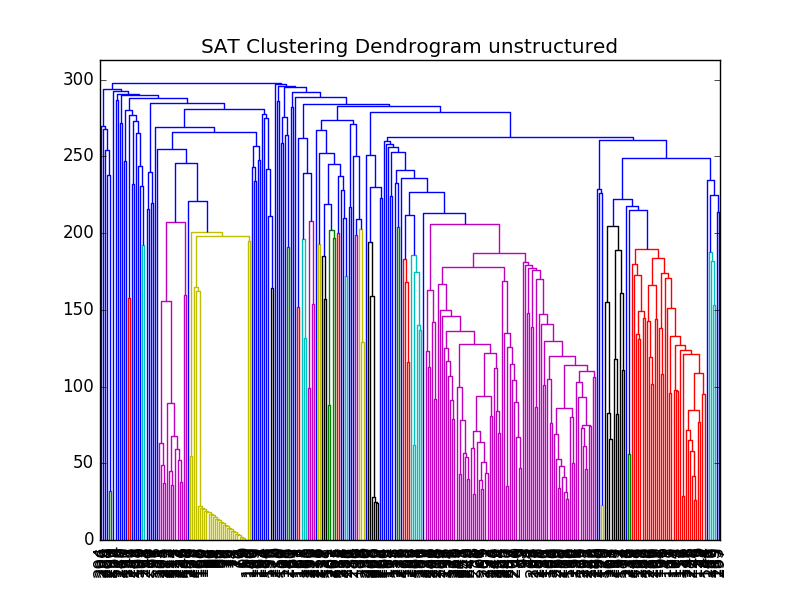
\includegraphics[scale=0.50]{../Pictures/SAT_Clustering_Dendrogram_unstructured.png}
\end{figure}

\begin{figure}
  \centering
  \caption{}
  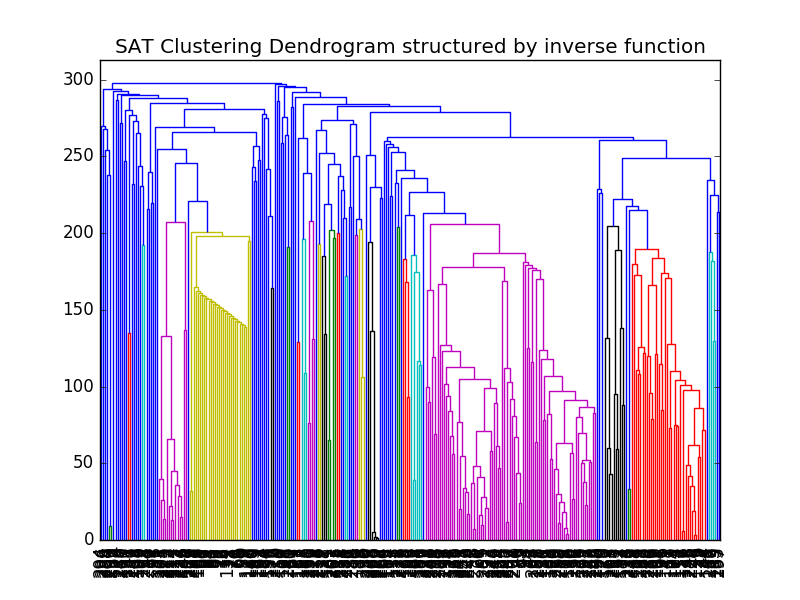
\includegraphics[scale=0.50]{../Pictures/SAT_Clustering_Dendrogram_structured_by_inverse_function.png}
\end{figure}

On peut remarquer que les deux figures sont presque identiques. Il y a différents clusters bien distincts, et en les étudiant de plus près, on note que ce sont effectivement les mêmes sur les deux figures. 
A priori, les associations faites par scikit correspondent bien à l'idée 
que nous nous faisions de benchmarks dont les résultats sont proches. Ces clusters pourrait permettre de constituer une première classification.
D'autre part il est aussi vérifiable des problèmes desquels on pourrait attendre qu'ils soient proches, comme les problèmes issus des mêmes milieux industriels, sont effectivement dans le même cluster.
Une approche simple pourrait aussi être de simplement regrouper les benchmarks de cette manière.

Seulement, nous aimerions savoir si ces différents clusters sont proches de des uns des autres ou forment de groupes bien définis. Or scikit-learn ne nous permet pas de récupérer la distance entre deux objets. 
Les figures 1 et 2 ne sont par conséquent pas de véritables dendrogrammes, mais des arbres permettant de visualiser les clusters. Afin de pouvoir mesurer la distance entre les cluster, nous avons utilisé une 
autre bibliothèque Python, \textit{scipy.cluster.hierarchy}. Grâce à cet outil, il est possible d'implémenter un clustering en utilisant la distance de notre choix. Nous allons donc pouvoir voir si il existe 
des  tendances consistantes à travers les différents distances utilisées, et si changer de distance, et donc d'approche, permet de faire émerger de nouvelles classes.

Pour commencer la figure 3 illustre le clustering opéré avec à l'aide de la distance euclidienne. Le dendrogramme est très différent de ceux étudiés précédemment. On peut remarquer qu'il n'y a pas de clusters 
très démarqués, et de manière générale, il y a peu de distance entre les différents clusters. Il semble donc difficile de définir des classes à partir de ce dendrogramme. D'autre part, il semblerait que des 
benchmarks issus des mêmes sources trouvent rarement ici dans les mêmes clusters. 

\begin{figure}
  \centering
  \caption{}
  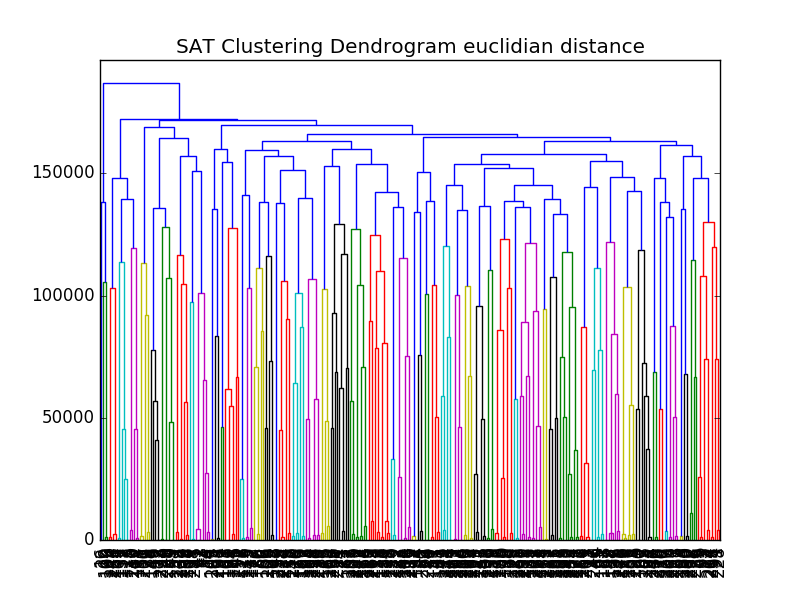
\includegraphics[scale=0.50]{../Pictures/SAT_Clustering_Dendrogram_euclidian_distance.png}
\end{figure}

La figure 4 présente le dendrogramme obtenue en utilisant la distance entre l’écart-type des résultats pour chaque benchmark. On note cette fois deux gros clusters, l'un, à droite, qui contient la majorité des 
benchmarks, tandis que celui de gauche en contient un petit nombre et semble être assez démarqué. Les benchmarks de ce groupe sont ceux ayant manifesté une grande variance par rapport aux résultats, il pourrait 
être intéressant de regarder si les performances d'un solveur sur ce petit groupe varient grandement lorsque l'on modifie le solveur.

\begin{figure}
  \centering
  \caption{}
  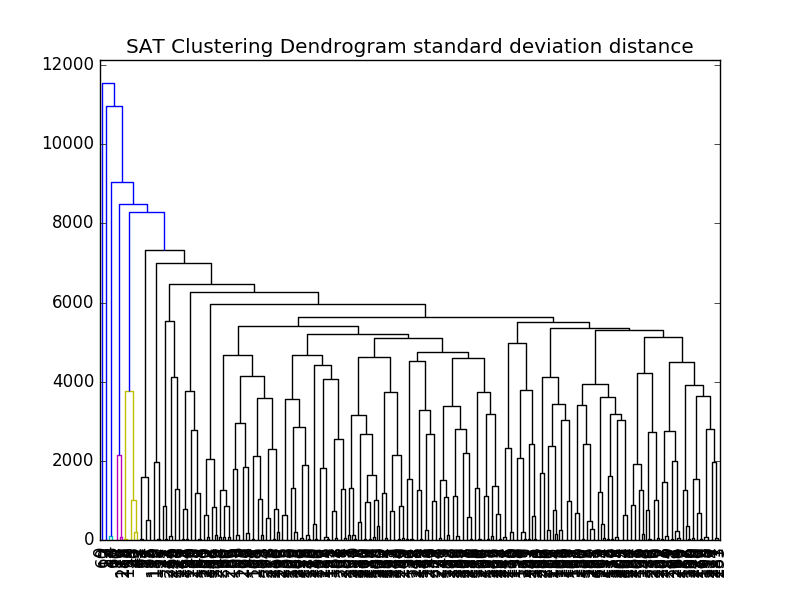
\includegraphics[scale=0.50]{../Pictures/SAT_Clustering_Dendrogram_average_standard_deviation_distance.png}
\end{figure}

Parmi les différentes approches proposées, il n'a pas été possible de discerner des groupes réduits que l'on pourrait considérer caractéristique d'un groupe plus globale, sauf peut-être le groupe à forte 
variance pour l'ensemble des benchmarks industriels, mais on ne sait pas encore s'il présente les caractéristiques recherchées.

\section{Exploitation des résultats et continuation}
\label{sec:validation}
Le Clustering nous offre la possibilité de distinguer un certain nombre de groupes de benchmarks qui pourraient avoir des propriétés communes. Il faudrait maintenant effectuer des tests spécifiques sur ces 
groupes. Par exemple, modifier les paramètres de certains solveurs pour voir si leurs performances évoluent de la même manière sur l'ensemble de ces groupes, et si certains groupes restent similaires après 
la modification d'une partie des solveurs. Malheureusement, nous n'avons pu nous intéresser qu'aux résultats statiques de la compétition.

Si ces résultats montrent que ces classes sont véritablement intéressantes, nous pourrions nous intéresser plus en détail à la recherche de problèmes caractéristiques. Pour repérer ceux-ci, il serait intéressant 
de chercher des critères permettrait de les identifier sans avoir à effectuer de tests supplémentaires. De manière alternative, il serait aussi possible d'identifier les problèmes caractéristiques directement par 
des tests : il existe des programmes, utilisés dans certaine compétitions de solveurs, qui permettent de régler les paramètres d'un solveur pour augmenter ses performances sur un groupe de problèmes particulier. 
Si on utilise un tel programme avec un groupe réduit de problèmes, et qu'on observe ensuite 'l'évolution des performances du solveur réglé sur le reste de la classe, on pourrait determiner si ce groupe est caractéristique.

\section{Conclusion}
\label{sec:conclusion}
Dans ce rapport nous avons pu aborder les problématiques liées à la recherche SAT et aux SAT-solvers. La compréhension de certains grands principes des algorithmes SAT et de la manière dont les performances des 
solveurs sont évaluées et améliorées permet de cerner l’intérêt d'une classification des problèmes SAT. L'utilisation des outils de machine learning a permis de mettre en avant des groupes de benchmarks qui 
présentent un intérêt à priori, les tests qui auraient permis d'établir si ces groupes peuvent permettre de dresser une classification  n'ont pas été effectué.
De plus seul un nombre réduit de clustering a été montré. En effet de nombreuses approches ont été essayées mais peu ont donné des résultats satisfaisants. 

Cependant les groupes qui ont été dégagés sont suffisants pour effectuer du travail supplémentaire et explorer la possibilité de créer une classification. Finalement la question reste encore ouverte car rien ne 
garantit pour l'instant qu'il soit possible de classifier les différents problèmes ou l'existence de problèmes caractéristiques. Le travail fourni jusqu'à présent nous offre cependant la possibilité de le vérifier 
de manière plus concrète.

% To use the English typographic conventions for the bibliography
\begin{otherlanguage}{english}
\printbibliography
\end{otherlanguage}

\end{document}



%%% Local Variables:
%%% mode: latex
%%% TeX-master: t
%%% End:
